\title{Lecture 7\\Representation of Parameters and Quantities in a Knowledge Base}

\begin{frame}
	\titlepage
\end{frame}

\begin{frame}{\\Lecture outline}
	\topline
	\justifying
	Scales, quantities and parameters. Measurable and non-measurable parameters. Exact, approximate and interval quantities. Connections with set cardinality, infinite sets and finite sets.
\end{frame}

%

\begin{frame}{\\Definition of a parameter}
	\topline
	\justifying
	\textbf{\textit{parameter}} is a class that is a family of all equivalence classes or tolerance classes defined by an equivalence relation or a tolerance relation.\\
\end{frame}

\begin{frame}{\\Definition of a parameter}
	\topline
	\justifying
	\begin{SCn}
		\scnheader{parameter}
		\scnidtf{characteristic}
		\scnidtf{property}
		\scnidtf{feature}
		\scnidtf{measurable property}
		\scnidtf{class of classes}
		\scnidtf{criterion for classifying or covering a class of entities}
		\scnidtf{criterion for partitioning or covering a class of entities}
		\scnidtf{family of sets that partition or cover a class of entities}
		\scnidtf{family of classes of entities with the same value of the corresponding property}
		\scnsuperset{directed parameter}
	\end{SCn}
\end{frame}

\begin{frame}{\\Types of parameters. Measurable parameter}
	\topline
	\justifying
	\begin{SCn}
		\scnheader{parameter}
		\begin{scnrelfromset}{\textit{partition}}
			\scnitem{measurable parameter}
			\scnitem{non-measurable parameter}
		\end{scnrelfromset}

		\scnheader{measurable parameter}
		\scnidtf{quantitative parameter}
		\scnidtf{family of measurable quantities}
		\scntext{explanation}{\footnotesize{Each \textbf{\textit{measurable parameter}} is a \textit{parameter} whose value (element, instance) is interpreted as a \textit{quantity} that can be assigned a numerical value using a chosen unit of measurement and/or reference point (the zero mark of the chosen scale).}}
		\scnsuperset{parameter measured on a scale}

	\end{SCn}
\end{frame}

\begin{frame}{\\Non-measurable parameter}
	\topline
	\justifying
	\begin{SCn}
		\scnheader{non-measurable parameter}
		\scnidtf{qualitative parameter}
	\end{SCn}
	\textbf{\textit{non-measurable parameter}} is a parameter for which no numerical equivalent and unit of measurement can be chosen. Examples include color and taste.
\end{frame}

\begin{frame}{\\}
	\topline
	\justifying
	\begin{SCn}
		\scnheader{parameter}
		\scntext{explanation}{\small{Each \textbf{\textit{parameter}} is a class that is a family of all equivalence classes or tolerance classes defined by either an \textit{equivalence relation} or a \textit{tolerance relation} (symmetric and reflexive, but only partially transitive).

For example, the elements (values, quantities) of the \textbf{\textit{parameter}} \textit{length} are either equivalence classes defined by the equivalence relation ``\textit{have exactly the same length*}'', tolerance classes defined by a relation of the form ``\textit{have approximately the same length to a specified accuracy*}'', or interval classes defined by binary relations of the form ``\textit{have a length within the same specified interval*}'' (for example, from 1 meter to 2 meters).}}
	\end{SCn}
\end{frame}


\begin{frame}{\\Parameter space}
	\topline
	\justifying
	\begin{SCn}
		\scnheader{parameter}
		\scntext{explanation}{\footnotesize{The elements (values, quantities) of a parameter may include intersecting sets (classes), but the union of all elements of each parameter is the class of all entities possessing that parameter (property, characteristic).

Each particular parameter (characteristic), i.e., each element of the class of all parameters, is a criterion for classifying entities that possess it according to equivalence (equality of its value).

A parameter may be partitioned into classes to refine a property. For example, the elements of the color parameter are classes corresponding to specific colors (blue, red, etc.). Each color may, in turn, include more specific classes, such as dark blue or light red.}
		}
	\end{SCn}
\end{frame}

\begin{frame}{\\Parameter space}
	\topline
	\justifying
	\begin{SCn}
		\scnheader{parameter}
		\scntext{explanation}{\footnotesize{In other words, each set of entities can be associated with a set (family) of parameters (a parameter space) possessed by those entities, analogous to a family of relations defined on that set. It is often useful to construct a parameter space whose ``points''{} correspond one-to-one to the entities being parameterized (for example, a set of parameters uniquely identifying each person).

Thus, for each used element (value) of a parameter, its specification must be stated explicitly: exact value, approximate value, interval value, accuracy or interval.}
		}
	\end{SCn}
\end{frame}

\begin{frame}{\\Parameter. Examples}
	\topline
	\justifying
	\vspace{10mm}
	\begin{figure}[H]
		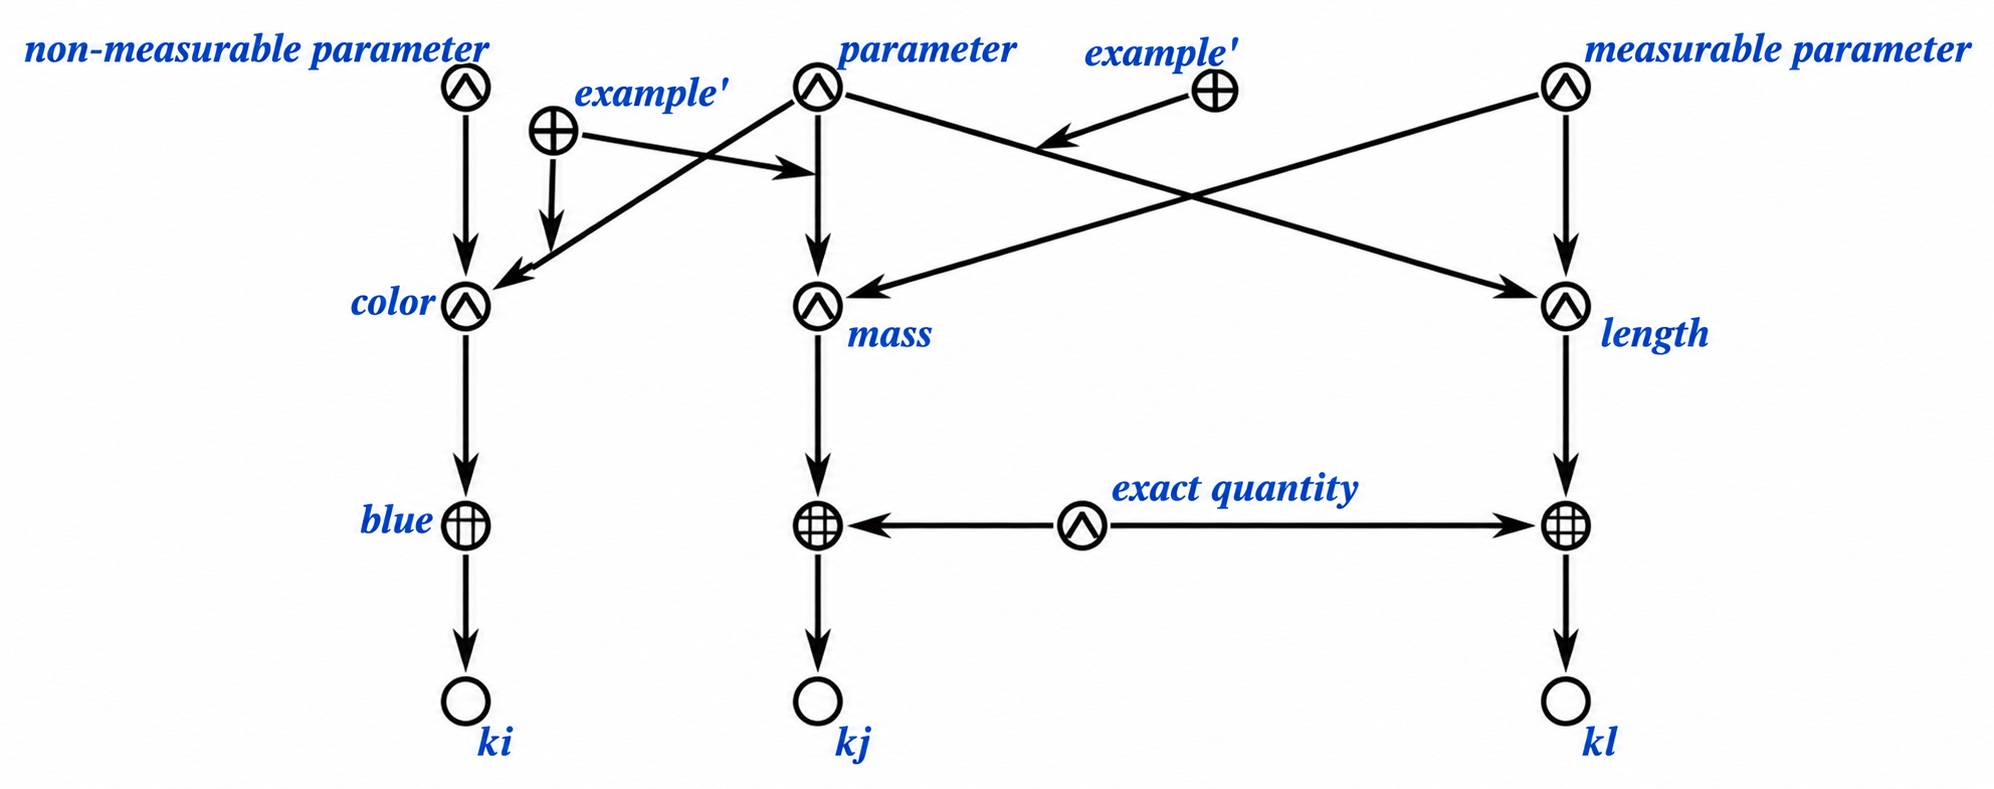
\includegraphics[width=0.94\linewidth,height=0.70\textheight,keepaspectratio]{./figures/sd_parameters/parameterDescription_en.png}
	\end{figure}
\end{frame}

\begin{frame}{\\Quantity}
	\topline
	\justifying
	\begin{SCn}
		\scnheader{quantity}
		\scnidtf{value of a quantitative parameter}
		\scnidtf{value of a measurable parameter}
		\scnidtf{class of entities with the same value of the corresponding parameter}
		\scnsuperset{exact quantity}
		\scnsuperset{approximate quantity}
		\scnsuperset{interval quantity}
	\end{SCn}
\end{frame}

\begin{frame}{\\Quantity}
	\topline
	\justifying
	\begin{SCn}
		\scnheader{quantity}
		\scntext{explanation}{\footnotesize{Each \textbf{\textit{quantity}} is an unambiguous measurement result for a characteristic of an entity, independent of the measurement scale.

Each \textbf{\textit{quantity}} can be assigned a numerical value using a chosen unit of measurement and reference point (the zero mark of the chosen scale, if measurement uses a scale).

The value of a parameter (a \textbf{\textit{quantity}}) must be distinguished from the value of that quantity on a scale, which may be scalar or vector-valued.}		}
	\end{SCn}
\end{frame}

\begin{frame}{\\Relation \textit{measurement*}}
	\topline
	\justifying
	\begin{SCn}
		\scnheader{measurement*}
		\scnidtf{parameter value*}
		\scnidtf{value of a given quantity of a given parameter*}
		\scnidtf{measurement as a correspondence*}
		\scnidtf{measurement result for a given quantity in a given unit and on a given scale*}
		\scnidtf{binary directed relation connecting quantities to their measurement results in various units and on various scales*}
	\end{SCn}
\end{frame}

\begin{frame}{\\Relation \textit{measurement*}}
	\topline
	\justifying
	\begin{SCn}
		\scnheader{measurement*}
		\scntext{explanation}{Tuples of the relation \textit{measurement*} connect a quantity to its value in a unit of measurement (including an interval value) or on a scale.

The specific unit or scale is additionally specified by the corresponding relation. A quantity can have only one value in each possible unit of measurement or one point on a given scale.}
	\end{SCn}
\end{frame}

\begin{frame}{\\Relation \textit{accuracy*}}
	\topline
	\justifying
	\begin{SCn}
		\scnheader{accuracy*}
		\scnidtf{deviation*}
		\scnidtf{accuracy of an approximate parameter value*}
		\scniselement{binary relation}
		\scntext{explanation}{Tuples of the relation \textbf{\textit{accuracy*}} connect an \textit{approximate quantity} to an \textit{exact quantity} of the same class that specifies the maximum possible deviation of the \textit{approximate quantity} from its value.}
	\end{SCn}
\end{frame}

\begin{frame}{\\Relation \textit{unit of measurement*}}
	\topline
	\justifying
	\begin{SCn}
		\scnheader{unit of measurement*}
		\scniselement{binary relation}
		\scnidtf{scale unit*}
		\scnidtf{unit mark on a scale*}
		\scntext{explanation}{Tuples of the relation \textbf{\textit{unit of measurement*}} connect the sign of a particular \textbf{\textit{measurement with a fixed unit}} to an \textit{exact quantity} belonging to the same particular \textit{parameter} as the first component of the tuples of that measurement, and used as the unit of measurement in this case.}
	\end{SCn}
\end{frame}

\begin{frame}{\\ \small{Measurement with a fixed unit}}
	\topline
	\justifying
	\begin{SCn}
		\scnheader{measurement with a fixed unit }
		\scnrelto{family of subsets}{measurement*}
		\scntext{explanation}{Each \textbf{\textit{measurement with a fixed unit}} is a subset of the relation \textit{measurement*} and is characterized by a \textit{unit of measurement*} that is an element of the same parameter (a family of entities whose value of that parameter equals the unit of measurement).}
	\end{SCn}
\end{frame}

\begin{frame}{\\Measurement on a scale}
	\topline
	\justifying
	\begin{SCn}
		\scnheader{measurement on a scale}
		\scnidtf{scale}
		\scnrelto{family of subsets}{measurement*}
		\scntext{explanation}{\small{Each \textbf{\textit{measurement on a scale}} is a subset of the relation \textit{measurement*} and is characterized by a reference point for that \textbf{\textit{scale}}.

The result of a \textbf{\textit{measurement on a scale}} is a point on the scale at a certain distance from the reference point in the required direction (lower or higher). This distance can be measured in any unit of measurement, while the quantity itself remains unchanged.}}
	\end{SCn}
\end{frame}

\begin{frame}{\\Measurement on a scale}
	\topline
	\justifying
	\begin{SCn}
		\scnheader{measurement on a scale}
		\scntext{explanation}{A \textbf{\textit{measurement on a scale}}, which depends on the \textit{zero mark*}, must be distinguished from measuring a change in the same \textit{parameter}, which is characterized by a unit of measurement and is independent of the reference point. For example, the date in a calendar corresponding to the \textit{start} of a process must be distinguished from the \textit{duration} of that process, which is independent of the chosen calendar.}
	\end{SCn}
\end{frame}

\begin{frame}{\\Measurement on a scale. Zero mark}
	\topline
	\justifying
	\begin{SCn}
		\scnheader{zero mark*}
		\scnidtf{zero on a scale*}
		\scnidtf{origin*}
		\scnidtf{reference point*}
		\scniselement{binary relation}
		\scntext{explanation}{Tuples of the relation \textbf{\textit{zero mark*}} connect the sign of a \textit{measurement on a scale} to the sign of an \textit{exact quantity} of the same \textit{parameter} that is taken as the reference point on the given scale.}
	\end{SCn}
\end{frame}

\begin{frame}{\\Measurement on a scale. Example}
	\topline
	\justifying
	\vspace{10mm}
	\begin{figure}[H]
		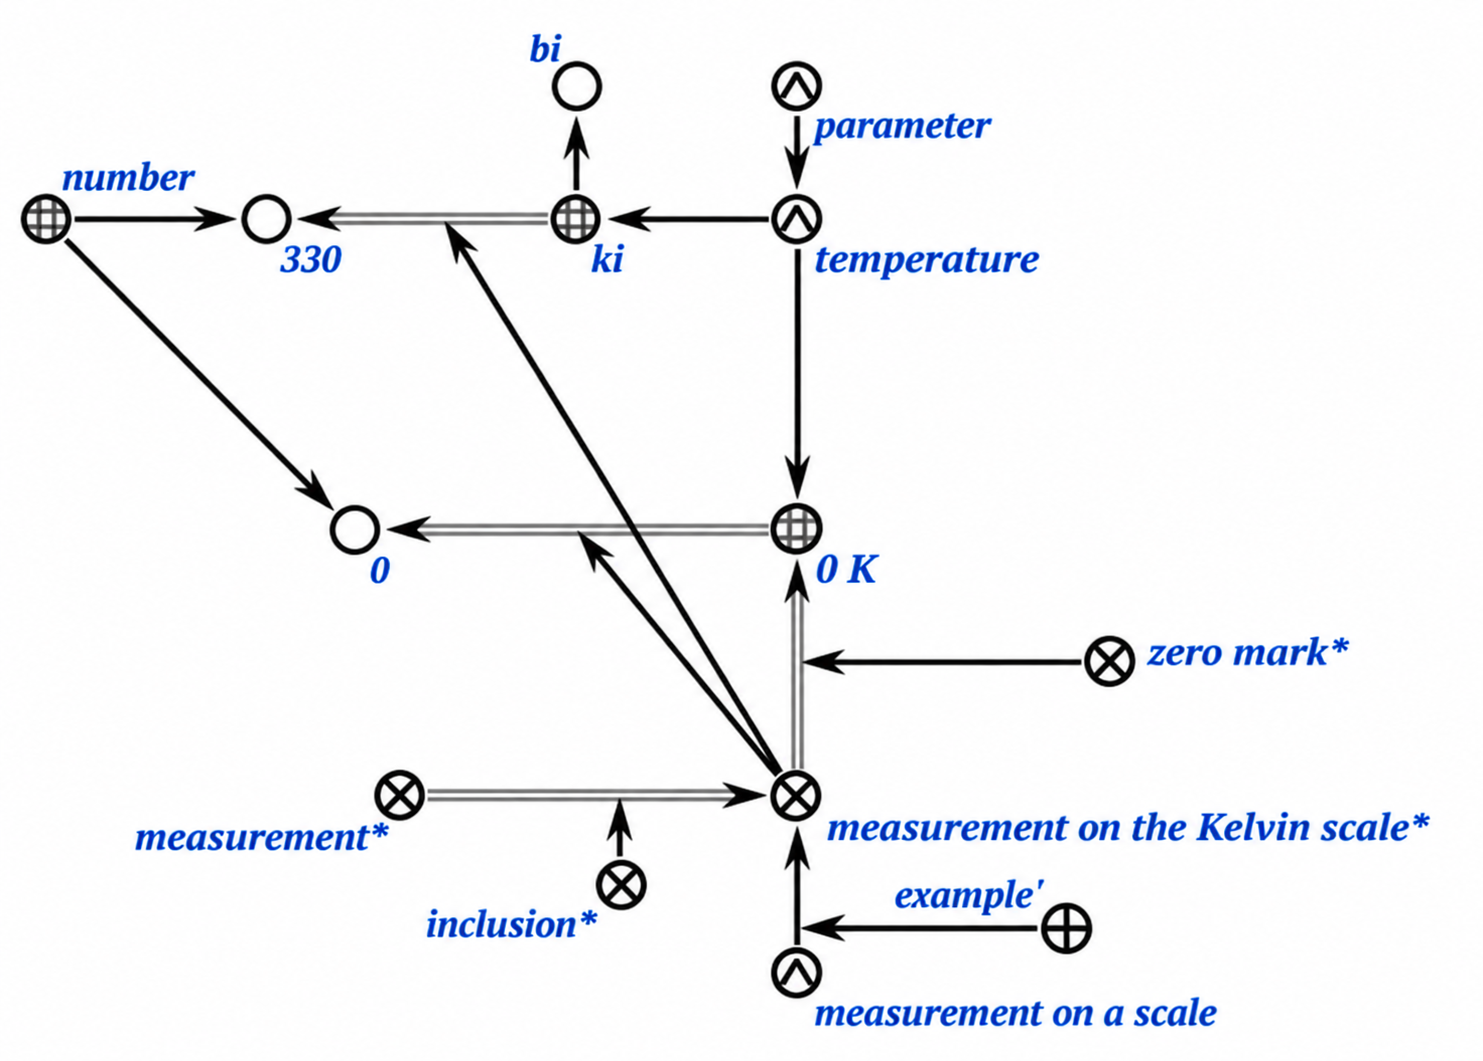
\includegraphics[height=188.475bp,keepaspectratio]{./figures/sd_parameters/scale_en.png}
	\end{figure}
\end{frame}

\begin{frame}{\\Exact quantity}
	\topline
	\justifying
	\begin{SCn}
		\scnheader{exact quantity}
		\scnidtf{exact parameter value}
		\scnidtf{set of all exact parameter values}
		\scnidtf{value of a parameter that is a family of equivalence classes corresponding to an equivalence relation}
		\scnidtf{equivalence class}
		\scntext{explanation}{\footnotesize{Each \textbf{\textit{exact quantity}} has a single fixed value in a unit of measurement or on a scale. All elements of this class are assumed to have the same value of the parameter, and deviations can be neglected.

Each \textbf{\textit{exact quantity}} can be associated with a group of \textit{approximate quantities} that are covers, rather than partitions, of the same set, with different degrees of accuracy.}}
	\end{SCn}
\end{frame}

\begin{frame}{\\Exact quantity. Example}
	\topline
	\justifying
	\vspace{10mm}
	\begin{figure}[H]
		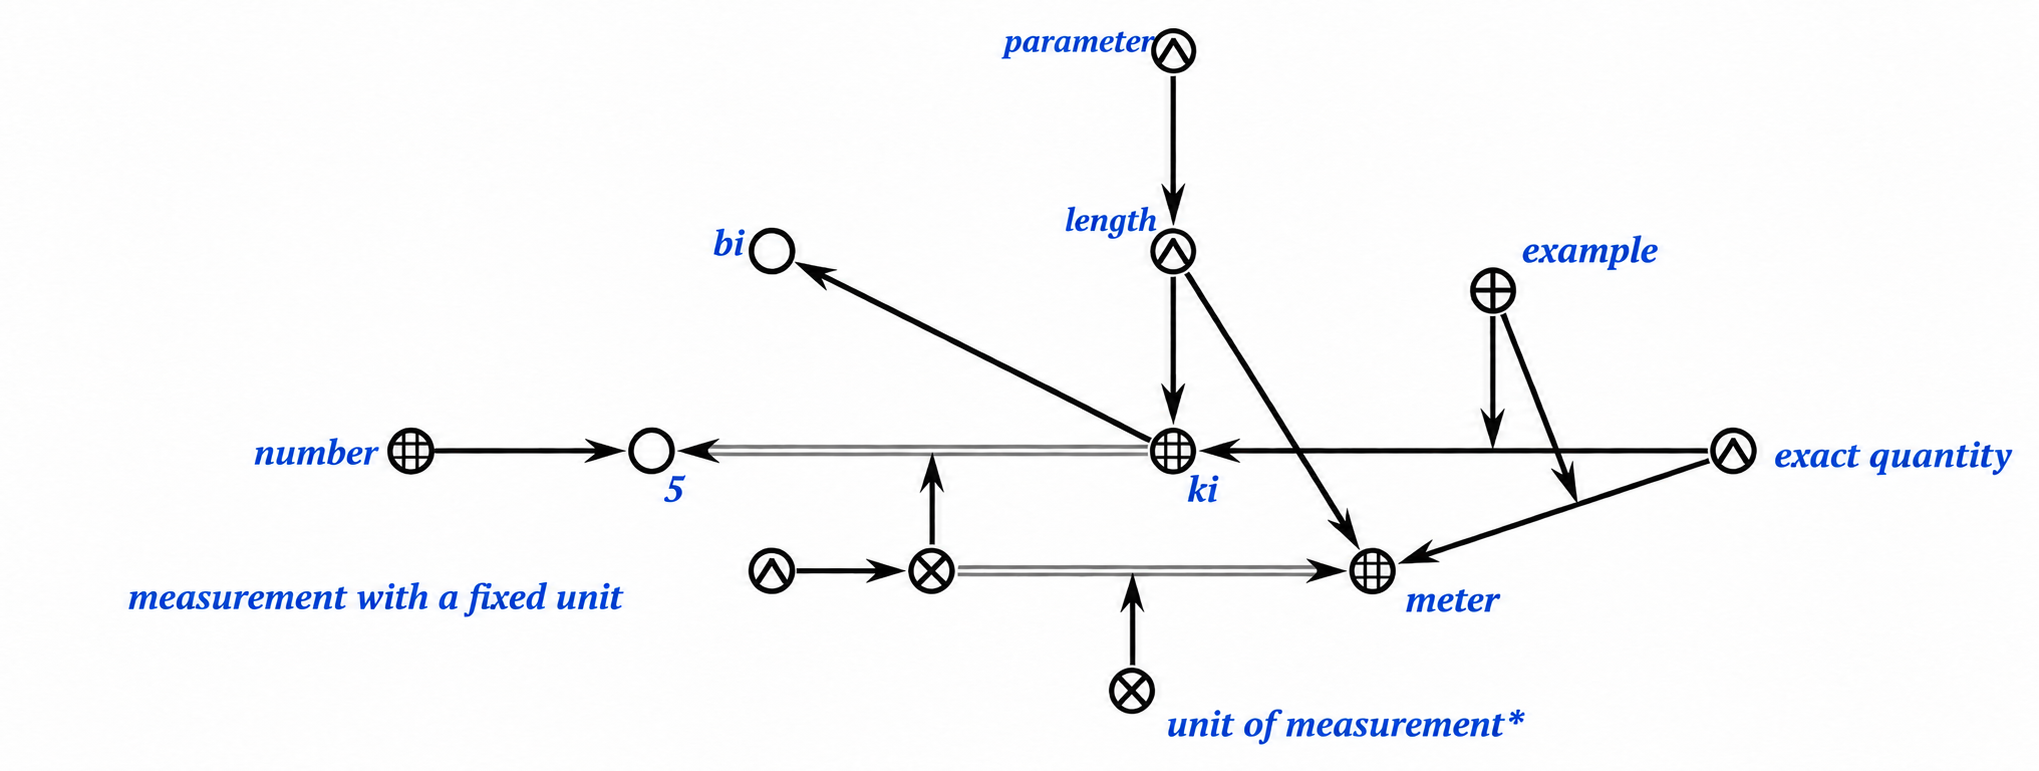
\includegraphics[width=0.94\linewidth,height=0.70\textheight,keepaspectratio]{./figures/sd_parameters/exactLength_en.png}
	\end{figure}
\end{frame}

\begin{frame}{\\Approximate quantity}
	\topline
	\justifying
	\begin{SCn}
		\scnheader{approximate quantity}
		\scnidtf{set of approximate parameter values}
		\scnidtf{approximate quantity}
		\scnidtf{approximate parameter value}
		\scnidtf{parameter value in an interval with unfixed bounds}
		\scntext{explanation}{\small{Each \textbf{\textit{approximate quantity}} is associated with its value in a unit of measurement or on a scale, and additionally with its \textit{accuracy*}, i.e., the possible deviation from that value.}}
	\end{SCn}
\end{frame}

\begin{frame}{\\Approximate quantity. Example}
	\topline
	\justifying
	\vspace{10mm}
	\begin{figure}[H]
		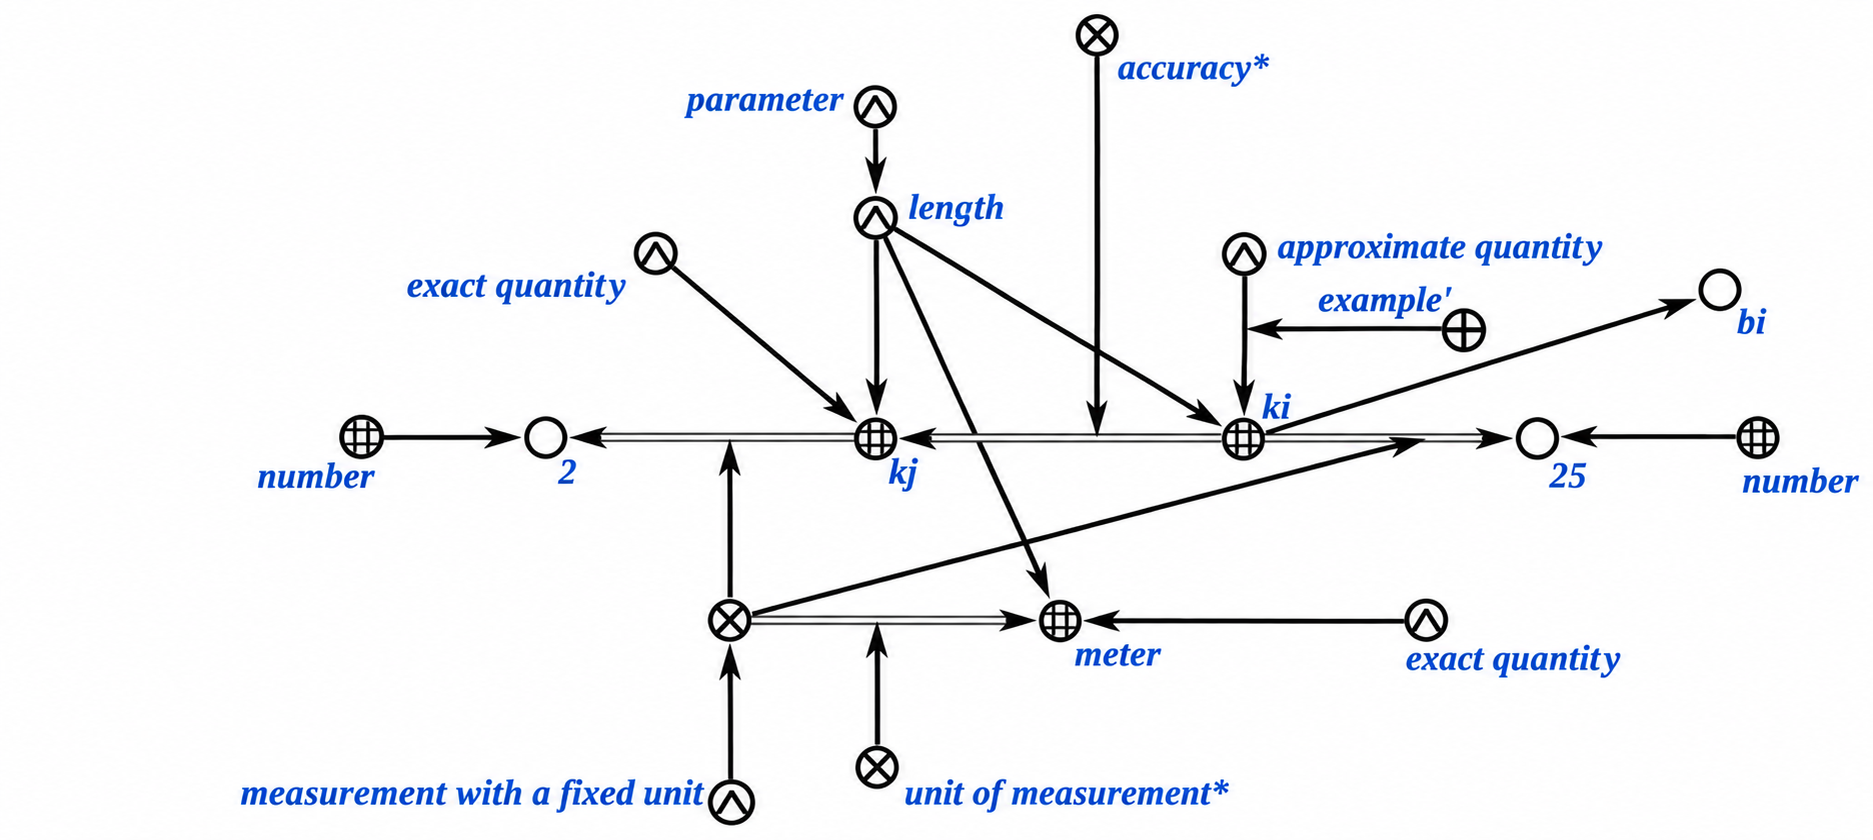
\includegraphics[width=0.94\linewidth,height=0.70\textheight,keepaspectratio]{./figures/sd_parameters/approximateLength_en.png}
	\end{figure}
\end{frame}

\begin{frame}{\\Interval quantity}
	\topline
	\justifying
	\begin{SCn}
		\scnheader{interval quantity}
		\scnidtf{interval parameter value}
		\scnidtf{parameter value in an interval with fixed bounds}
		\scnidtf{parameter-value interval from a set of overlapping intervals of different lengths with unfixed bounds}
		\scntext{explanation}{\small{Each \textbf{\textit{interval quantity}} is a class of entities within a precisely specified interval whose minimum and maximum points are \textit{exact quantities}. The result of \textit{measurement*} of such a quantity is an ordered pair whose first component is the left (lower) bound and whose second component is the right (upper) bound of the interval.}}
	\end{SCn}
\end{frame}

\begin{frame}{\\Interval quantity. Example}
	\topline
	\justifying
	\vspace{10mm}
	\begin{figure}[H]
		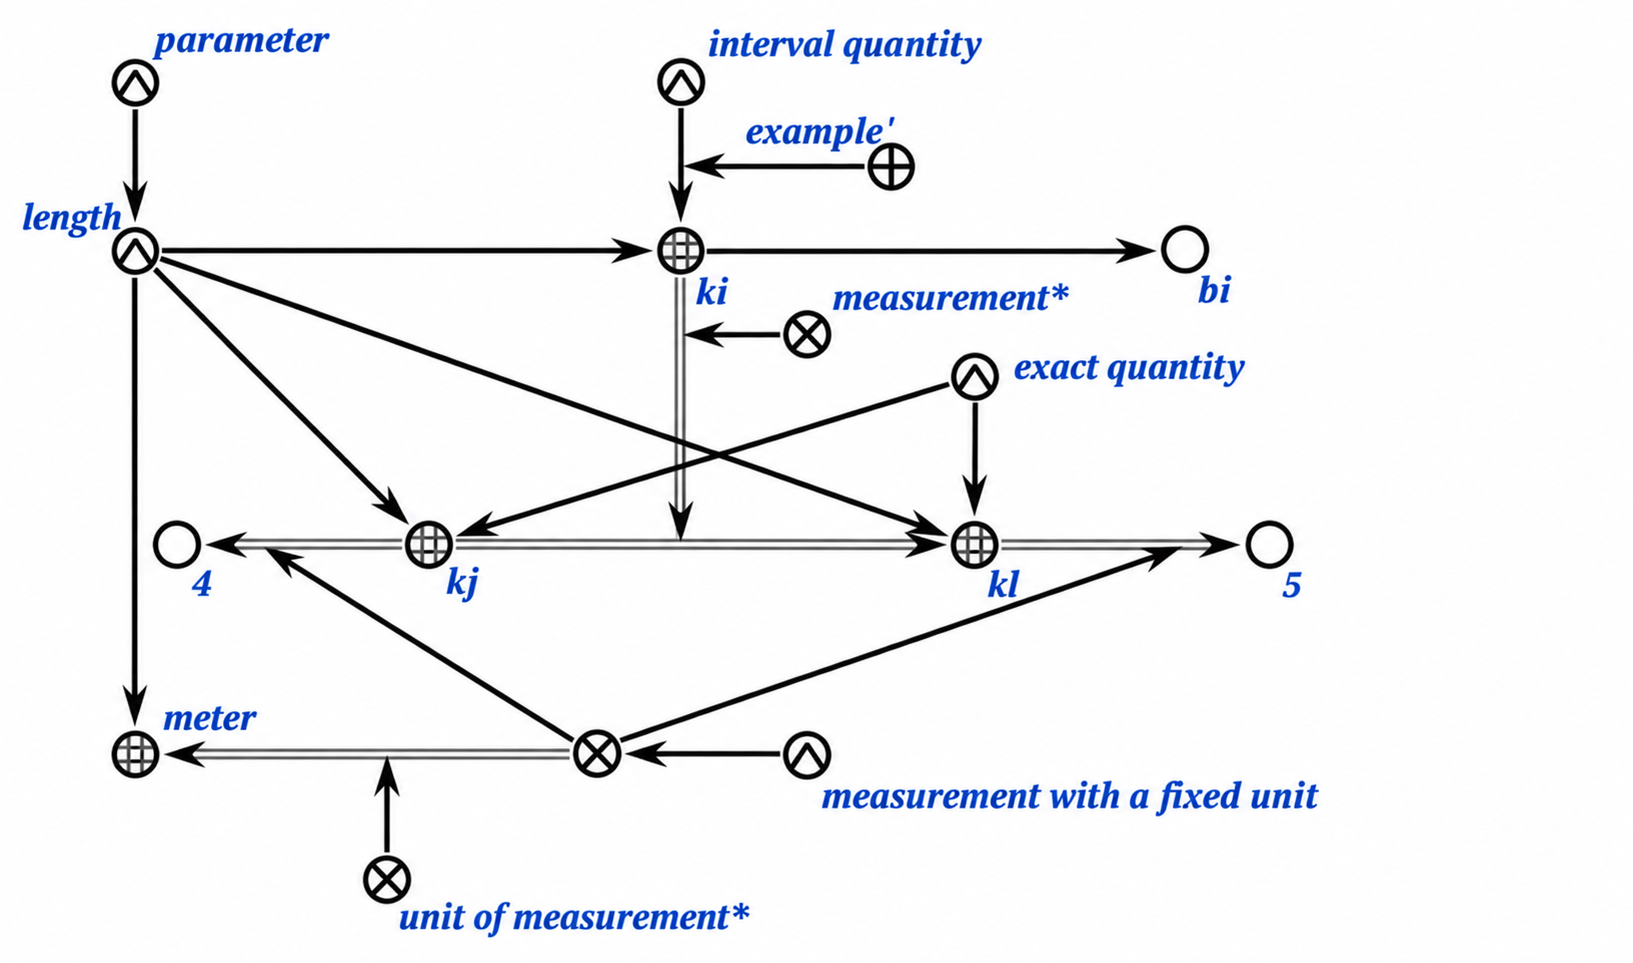
\includegraphics[height=180.6bp,keepaspectratio]{./figures/sd_parameters/intervalLength_en.png}
	\end{figure}
\end{frame}

\begin{frame}{\\Measurement as an action}
	\topline
	\justifying
	\begin{SCn}
		\scnheader{action. measurement}
		\scnidtf{measurement as an action}
		\scnidtf{action aimed at establishing a connection belonging to the measurement* relation between a quantity of a given parameter, to which a given entity belongs, and the corresponding value of that quantity on a scale}
		\scnidtf{action aimed at solving the task of measuring a given parameter of a given entity}
		\scnsubset{action}
	\end{SCn}
\end{frame}

\begin{frame}{\\Measurement as a task}
	\topline
	\justifying
	\begin{SCn}
		\scnheader{task. measurement}
		\scnidtf{specification of a measurement action}
		\scnidtf{specification of an action aimed at measuring a given parameter of a given entity}
		\scnsubset{task}
	\end{SCn}
\end{frame}
